% =============================================================================
% serial_learning_material.tex
% Learning Material: Serial Baseline & Algorithm Foundation
% EC7207 High Performance Computing – Group 11
% =============================================================================
\documentclass[12pt,a4paper]{article}

\usepackage[margin=2.5cm]{geometry}
\usepackage{listings}
\usepackage{xcolor}
\usepackage{amsmath}
\usepackage{amssymb}
\usepackage{booktabs}
\usepackage{hyperref}
\usepackage{tikz}
\usepackage{array}
\usepackage{enumitem}
\usepackage{fancyhdr}
\usepackage{titlesec}

% ── Code listing style ────────────────────────────────────────────────────────
\lstdefinestyle{cstyle}{
    language=C,
    basicstyle=\ttfamily\small,
    keywordstyle=\color{blue}\bfseries,
    commentstyle=\color{gray}\itshape,
    stringstyle=\color{red!70!black},
    numbers=left, numberstyle=\tiny\color{gray},
    numbersep=8pt, frame=single, rulecolor=\color{black!30},
    breaklines=true, showstringspaces=false,
    backgroundcolor=\color{gray!5},
    tabsize=4
}
\lstset{style=cstyle}

% ── Header / Footer ───────────────────────────────────────────────────────────
\pagestyle{fancy}
\fancyhf{}
\lhead{EC7207 HPC – Group 11}
\rhead{Serial Baseline \& Algorithm Foundation}
\cfoot{\thepage}

\titleformat{\section}{\large\bfseries}{}{0em}{}[\titlerule]
\titleformat{\subsection}{\normalsize\bfseries}{}{0em}{}

% =============================================================================
\begin{document}
% =============================================================================

\begin{center}
    {\LARGE\bfseries Serial Baseline \& Algorithm Foundation}\\[0.5em]
    {\large Learning Material for EC7207 High Performance Computing}\\[0.3em]
    {\normalsize Group 11 — Pearson Correlation Recommender System}
\end{center}
\vspace{1em}
\hrule
\vspace{1.5em}

% =============================================================================
\section{Why We Start With a Serial Version}
% =============================================================================

Before parallelising \emph{anything}, every HPC project must have a correct
serial implementation.  This serial version serves three fundamental roles:

\begin{enumerate}
    \item \textbf{Correctness baseline} — Every parallel version (OpenMP,
          Pthreads, MPI, CUDA, Hybrid) must produce the same numerical results.
          If a parallel version's Mean Absolute Error (MAE) differs by more than
          $\pm 0.001$ from the serial result, there is a race condition or a
          distribution bug.
    \item \textbf{Speedup denominator} — Speedup is defined as
          $S = T_{\text{serial}} / T_{\text{parallel}}$.  Without a reliable
          serial time $T_{\text{serial}}$, speedup cannot be computed.
    \item \textbf{Algorithm clarity} — A serial version expresses the algorithm
          without the extra complexity of synchronisation primitives.  Read this
          file first, then study the parallel versions to see only what changed.
\end{enumerate}

\begin{center}
\fbox{\parbox{0.88\textwidth}{
\textbf{Key Rule:}  The serial version uses \texttt{srand(SEED)} with
\texttt{SEED = 42}.  Every parallel version does the same.  This guarantees
all versions operate on \emph{identical} data, making comparisons fair.
}}
\end{center}

% =============================================================================
\section{The Recommendation Problem}
% =============================================================================

\subsection{User-Based Collaborative Filtering}

Our program implements \textbf{User-Based Collaborative Filtering (CF)}, the
fundamental technique behind systems like Netflix, Spotify, and Amazon
recommendations.

\textbf{The core idea:}  If User~A and User~B have rated many items similarly
in the past, then when User~A rates a new item, User~B's predicted rating for
that item should be close to User~A's actual rating.

\medskip
\textbf{Data structure — ratings matrix $R$:}

\[
R =
\begin{pmatrix}
4 & 0 & 2 & 5 & 0 \\
0 & 3 & 0 & 4 & 1 \\
5 & 0 & 3 & 0 & 2 \\
0 & 2 & 4 & 0 & 5 \\
\end{pmatrix}
\quad
\begin{array}{l}
\leftarrow \text{User 0} \\
\leftarrow \text{User 1} \\
\leftarrow \text{User 2} \\
\leftarrow \text{User 3}
\end{array}
\]

\begin{itemize}
    \item Rows = users, Columns = items (movies, songs, products, \ldots)
    \item $R_{u,i} = 0$ means user $u$ has not rated item $i$ (unknown)
    \item $R_{u,i} \in \{1,2,3,4,5\}$ means user $u$ rated item $i$
    \item \textbf{Goal:} Fill in the zeros — predict what each user would rate items they haven't seen
\end{itemize}

\subsection{Matrix Storage: Flat 1-D Arrays (Row-Major)}

In our project, a 2-D matrix $M[\text{row}][\text{col}]$ is stored as a single
flat array in \emph{row-major} order — the same way C stores 2-D arrays:

\[
\text{flat}[r \times \text{num\_cols} + c] = M[r][c]
\]

\begin{lstlisting}
/* Project macros — convert (row,col) to flat index */
#define R(u,i)    ratings[(u)*N_ITEMS  + (i)]
#define SIM(u,v)  sim_matrix[(u)*N_USERS + (v)]
#define PRED(u,i) predictions[(u)*N_ITEMS + (i)]
\end{lstlisting}

\textbf{Why?}  A single \texttt{malloc} call is simpler and more cache-friendly
than arrays of pointers.  Adjacent elements in a row are contiguous in memory,
which maximises CPU cache utilisation during row scans.

% =============================================================================
\section{Pearson Correlation — The Similarity Measure}
% =============================================================================

\subsection{The Formula}

The \textbf{Pearson Correlation Coefficient} between users $u$ and $v$ is:

\[
\text{sim}(u,v) = \frac
{ \displaystyle\sum_{i \in I_{uv}} (R_{u,i} - \bar{R}_u)\,(R_{v,i} - \bar{R}_v) }
{ \sqrt{\displaystyle\sum_{i \in I_{uv}} (R_{u,i} - \bar{R}_u)^2} \;\times\;
  \sqrt{\displaystyle\sum_{i \in I_{uv}} (R_{v,i} - \bar{R}_v)^2} }
\]

where:
\begin{itemize}
    \item $I_{uv}$ = set of items rated by \textbf{both} $u$ and $v$
          (co-rated items)
    \item $\bar{R}_u$ = mean rating of user $u$ (computed in Phase~2)
    \item $\bar{R}_v$ = mean rating of user $v$
\end{itemize}

\subsection{Interpretation}

\begin{center}
\begin{tabular}{cl}
\toprule
Value & Meaning \\
\midrule
$+1.0$ & Perfect agreement — users rate everything identically \\
$0.0$  & No relationship \\
$-1.0$ & Perfect disagreement — one rates high where other rates low \\
\bottomrule
\end{tabular}
\end{center}

\subsection{Why Subtract the Mean?}

Without mean-subtraction, an optimistic user who rates everything 5 would
appear similar to anyone, regardless of taste.  By working with
\emph{deviations} $(R_{u,i} - \bar{R}_u)$, Pearson captures \emph{relative
preference} — how much above or below their own average a user rates each item.

\subsection{Edge Cases in the Code}

\begin{lstlisting}
static float pearson_similarity(int u, int v)
{
    /* ... accumulate num, den_u, den_v, co ... */

    if (co < 2) return 0.0f;         /* need >= 2 co-rated items */
    double denom = sqrt(den_u) * sqrt(den_v);
    if (denom < 1e-10) return 0.0f;  /* zero variance -> undefined */

    float s = (float)(num / denom);
    if (s >  1.0f) s =  1.0f;        /* clamp floating-point overshoot */
    if (s < -1.0f) s = -1.0f;
    return s;
}
\end{lstlisting}

\begin{itemize}
    \item \textbf{co $<$ 2}: One co-rated item gives a trivially perfect or
          $-1$ correlation that is statistically meaningless.
    \item \textbf{denom $\approx$ 0}: One user gave the same rating to all
          co-rated items (zero variance) — correlation is undefined, return 0.
    \item \textbf{Clamping}: Floating-point arithmetic can produce values like
          $1.0000001$ due to rounding — clamping keeps the result in $[-1,1]$.
\end{itemize}

% =============================================================================
\section{The 5-Phase Algorithm}
% =============================================================================

\begin{center}
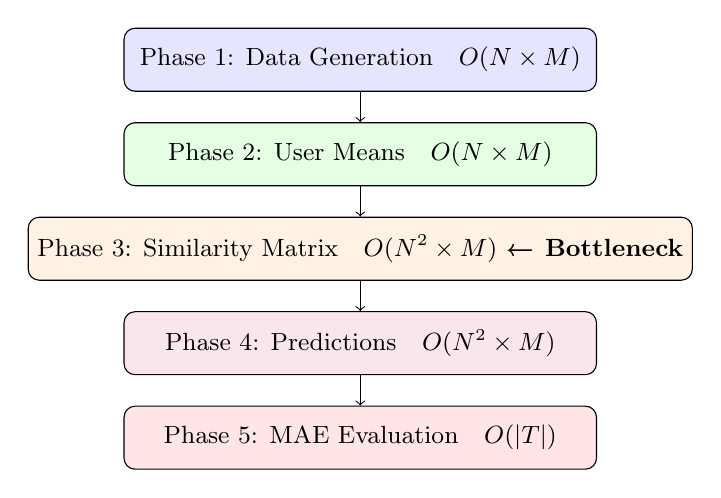
\begin{tikzpicture}[node distance=1.2cm,
    box/.style={rectangle, draw, rounded corners, minimum width=6cm,
                minimum height=0.8cm, text centered, font=\small}]
    \node[box, fill=blue!10]  (p1) {Phase 1: Data Generation\quad $O(N \times M)$};
    \node[box, fill=green!10] (p2) [below of=p1] {Phase 2: User Means\quad $O(N \times M)$};
    \node[box, fill=orange!10](p3) [below of=p2] {Phase 3: Similarity Matrix\quad $O(N^2 \times M)$ \textbf{← Bottleneck}};
    \node[box, fill=purple!10](p4) [below of=p3] {Phase 4: Predictions\quad $O(N^2 \times M)$};
    \node[box, fill=red!10]   (p5) [below of=p4] {Phase 5: MAE Evaluation\quad $O(|T|)$};
    \draw[->] (p1)--(p2); \draw[->] (p2)--(p3);
    \draw[->] (p3)--(p4); \draw[->] (p4)--(p5);
\end{tikzpicture}
\end{center}

\subsection{Phase 1 — Data Generation}

Synthetic data is generated with a \emph{three-dice} process for each
$(u, i)$ cell:

\begin{enumerate}
    \item \textbf{Sparsity die}: with probability 0.70, skip cell (unrated)
    \item \textbf{Rating die}: assign rating $= (\text{rand()} \% 5) + 1 \in \{1,2,3,4,5\}$
    \item \textbf{Split die}: with probability 0.10, move to test set (hidden
          during training, used only for MAE evaluation)
\end{enumerate}

\begin{lstlisting}
srand(SEED);  /* SEED=42 -- deterministic, same data every run */
for (int u = 0; u < N_USERS; u++) {
    for (int i = 0; i < N_ITEMS; i++) {
        if ((float)rand() / RAND_MAX < SPARSITY) continue;  /* die 1 */
        float rating = (float)(rand() % 5) + 1.0f;           /* die 2 */
        if ((float)rand() / RAND_MAX < TEST_RATIO) {
            /* die 3: hold out for evaluation */
            test_set[test_size++] = (TestEntry){u, i, rating};
        } else {
            R(u, i) = rating;  /* training data */
        }
    }
}
\end{lstlisting}

\subsection{Phase 2 — User Means}

$\bar{R}_u = \frac{1}{|\{i : R_{u,i} \neq 0\}|} \sum_{i: R_{u,i} \neq 0} R_{u,i}$

If a user has rated nothing, default to 3.0 (mid-scale of $[1,5]$).

\subsection{Phase 3 — Similarity Matrix (Bottleneck)}

\begin{lstlisting}
/* Upper-triangle strategy: sim(u,v) == sim(v,u), compute once */
for (int u = 0; u < N_USERS; u++) {
    SIM(u, u) = 1.0f;             /* self-similarity = 1 by definition */
    for (int v = u + 1; v < N_USERS; v++) {
        float s = pearson_similarity(u, v);
        SIM(u, v) = s;            /* upper triangle */
        SIM(v, u) = s;            /* lower triangle mirror */
    }
}
\end{lstlisting}

\textbf{Why is this the bottleneck?}
\begin{itemize}
    \item $N_{\text{USERS}}(N_{\text{USERS}}-1)/2$ unique pairs to evaluate
    \item For $N = 1000$: $499{,}500$ Pearson calls, each scanning up to
          1000 items $\approx 500\,\text{M}$ floating-point operations
    \item This is what all parallel versions accelerate
\end{itemize}

\subsection{Phase 4 — Predictions}

\[
\text{pred}(u,i) = \bar{R}_u +
\frac{\displaystyle\sum_{k \in K} \text{sim}(u,k) \cdot (R_{k,i} - \bar{R}_k)}
     {\displaystyle\sum_{k \in K} \text{sim}(u,k)}
\]

where $K$ = top-\texttt{TOP\_K} (20) most similar neighbours who have rated item $i$ with positive similarity.

\textbf{Intuition:}  Start from user $u$'s average.  Adjust upward if
similar neighbours liked the item above their own average; adjust downward
if they disliked it.

\begin{lstlisting}
/* Collect positive-sim neighbours who rated this item */
int cnt = 0;
for (int v = 0; v < N_USERS; v++) {
    if (v == u || R(v, item) == 0.0f) continue;
    float s = SIM(u, v);
    if (s <= 0.0f) continue;      /* only positive similarity */
    nbrs[cnt++] = (SimPair){v, s};
}
/* Sort descending by similarity, take best TOP_K */
qsort(nbrs, cnt, sizeof(SimPair), cmp_sim_desc);
int k = (cnt < TOP_K) ? cnt : TOP_K;
\end{lstlisting}

\subsection{Phase 5 — MAE Evaluation}

\[
\text{MAE} = \frac{1}{|T|} \sum_{(u,i) \in T} |\text{pred}(u,i) - R_{u,i}^{\text{actual}}|
\]

MAE is in the same units as ratings (1–5 scale). Lower is better.
A MAE of 0.5 means predictions are off by half a star on average.

% =============================================================================
\section{Performance Concepts}
% =============================================================================

\subsection{Time Complexity}

\begin{center}
\begin{tabular}{lll}
\toprule
Phase & Complexity & For $N=1000, M=1000$ \\
\midrule
Data Generation & $O(N \times M)$ & $10^6$ operations \\
User Means      & $O(N \times M)$ & $10^6$ operations \\
Similarity      & $O(N^2 \times M)$ & $\approx 500 \times 10^6$ \\
Predictions     & $O(N^2 \times M)$ & $\approx 500 \times 10^6$ \\
MAE             & $O(|T|)$          & $\approx 30{,}000$ \\
\bottomrule
\end{tabular}
\end{center}

Phases 3 and 4 dominate.  Parallelism targets these two phases.

\subsection{Timing in the Serial Version}

\begin{lstlisting}
/* clock_gettime(CLOCK_MONOTONIC) is monotonic (never goes backwards) */
static double now_sec(void) {
    struct timespec ts;
    clock_gettime(CLOCK_MONOTONIC, &ts);
    return ts.tv_sec + ts.tv_nsec * 1e-9;
}
/* Usage: t0 = now_sec(); ... work ... t1 = now_sec() - t0; */
\end{lstlisting}

\textbf{Why not \texttt{clock()}?}  \texttt{clock()} measures \emph{CPU time}
summed across all threads.  For parallel versions with 4 threads, it would
report $4\times$ the wall-clock time.  \texttt{CLOCK\_MONOTONIC} measures
actual elapsed (wall-clock) time, which is what speedup calculations need.

\subsection{Output Format for Automated Parsing}

All versions emit tagged lines that the benchmark script parses:
\begin{verbatim}
[Data]   Users: 1000 | Items: 1000 | Sparsity: 70% | Test ratings: 30012
[Timing] Similarity matrix  : 12.3456 s
[Timing] Prediction phase   : 8.7654 s
[Check]  Sim-matrix checksum: 12345.678901
[Eval]   MAE on test set    : 0.4523  (test size: 30012)
[Timing] Total (sim+pred)   : 21.1110 s
\end{verbatim}

\begin{itemize}
    \item \texttt{[Timing]} lines are parsed by the benchmark script to compute speedup
    \item \texttt{[Check]} line = sum of all $N^2$ similarity values;
          must match across all CPU versions
    \item \texttt{[Eval]} line = MAE; must match within $\pm 0.001$
\end{itemize}

% =============================================================================
\section{Speedup and Efficiency — Theory}
% =============================================================================

These formulas apply across all parallel versions.  The serial version provides
$T_{\text{serial}}$ for all calculations.

\subsection{Amdahl's Law}

If fraction $f$ of a program \emph{cannot} be parallelised:

\[
S_{\max}(p) = \frac{1}{f + (1-f)/p}
\quad \xrightarrow{p \to \infty} \quad \frac{1}{f}
\]

\textbf{Example:} If Phase~1 (data generation, serial) takes 5\% of total
time, $f = 0.05$, so $S_{\max} = 20$.  No matter how many cores you add,
you cannot go faster than $20\times$.

\subsection{Speedup and Efficiency}

\[
\text{Speedup}(p) = \frac{T_{\text{serial}}}{T_{\text{parallel}}(p)}
\qquad
\text{Efficiency}(p) = \frac{\text{Speedup}(p)}{p} \in (0, 1]
\]

\begin{itemize}
    \item Efficiency = 1.0 means \emph{perfect} linear speedup (ideal)
    \item Efficiency $< 1.0$ due to overhead: synchronisation, communication,
          load imbalance, serial fractions
    \item Efficiency $> 1.0$ (\emph{superlinear}) occasionally occurs due to
          cache effects (problem now fits in L3 per core)
\end{itemize}

\subsection{Where to See This in Our Project}

The \texttt{results/speedup\_table.csv} file records these values for all
versions and thread/process counts.  The \texttt{results/run\_benchmarks.sh}
script computes them automatically:

\begin{verbatim}
speedup   = SERIAL_TOTAL / total
efficiency = speedup / workers
\end{verbatim}

% =============================================================================
\section{Key Things to Explain in a Presentation}
% =============================================================================

\begin{enumerate}
    \item \textbf{Why fixed seed?}  So all versions see the same data and MAE
          comparisons are meaningful.
    \item \textbf{Why Pearson and not cosine similarity?}  Pearson is
          mean-centred, so it is robust to users with different rating biases.
          Cosine similarity does not subtract the mean.
    \item \textbf{Why upper-triangle only?}  $\text{sim}(u,v) = \text{sim}(v,u)$
          (symmetric), so computing both would waste exactly half the work.
    \item \textbf{Why \texttt{calloc} not \texttt{malloc}?}  \texttt{calloc}
          zero-initialises, and $0.0$ is our sentinel for ``unrated.''
    \item \textbf{Why store the test set separately?}  We need to hide those
          ratings from the similarity and prediction algorithms, then use them
          to measure how accurately we predicted.
    \item \textbf{Why TOP\_K = 20?}  Using all $N-1$ neighbours is noisy;
          restricting to the top 20 most similar neighbours improves accuracy
          and reduces computation.
\end{enumerate}

% =============================================================================
\section{Compile and Run}
% =============================================================================

\begin{verbatim}
# Compile
gcc -O2 -Wall -o serial_rec serial/serial_recommender.c -lm

# Run (default 1000 users, 1000 items)
./serial_rec

# Custom size
./serial_rec 500 300
./serial_rec 2000 1500
\end{verbatim}

\textbf{Flags:}
\begin{itemize}
    \item \texttt{-O2}: optimisation level 2 (enables vectorisation, loop unrolling, etc.)
    \item \texttt{-Wall}: enable all warnings (good practice)
    \item \texttt{-lm}: link the math library (required for \texttt{sqrt}, \texttt{fabs})
\end{itemize}

\vfill
\begin{center}
    \small\textit{Group 11 — EC7207 High Performance Computing}
\end{center}

\end{document}
